\documentclass[12pt]{article}
\usepackage[margin=1.5cm]{geometry}
\usepackage{parskip}
\usepackage{amsmath}
\usepackage{amssymb}
\usepackage{amsfonts}
\usepackage{enumitem}
\usepackage{graphicx}
\usepackage{stmaryrd}
\graphicspath{ {./images/} }


\begin{document}
\begin{enumerate}[label=(\alph*)]

  \item
    We give the following expressions:

    $I(X;Y) = H(Y|X) - H(Y)$

    $I(X;Y) = H(X|Y) - H(X)$

    $I(X;Y) = H(X) + H(Y) - H(X,Y)$

    In ordinary terms, $H(X|Y)$ denotes how much uncertainty there is left in $X$ after learning the value of $Y$.

    $H(X)$ denotes how much uncertainty there is in knowing the value of $X$.

    $H(X,Y)$ denotes how much uncertainty there is in knowing both the value of $X$ and $Y$

    $I(X;Y)$ denotes how much information $X$ and $Y$ have in common

    A diagram is drawn below:

    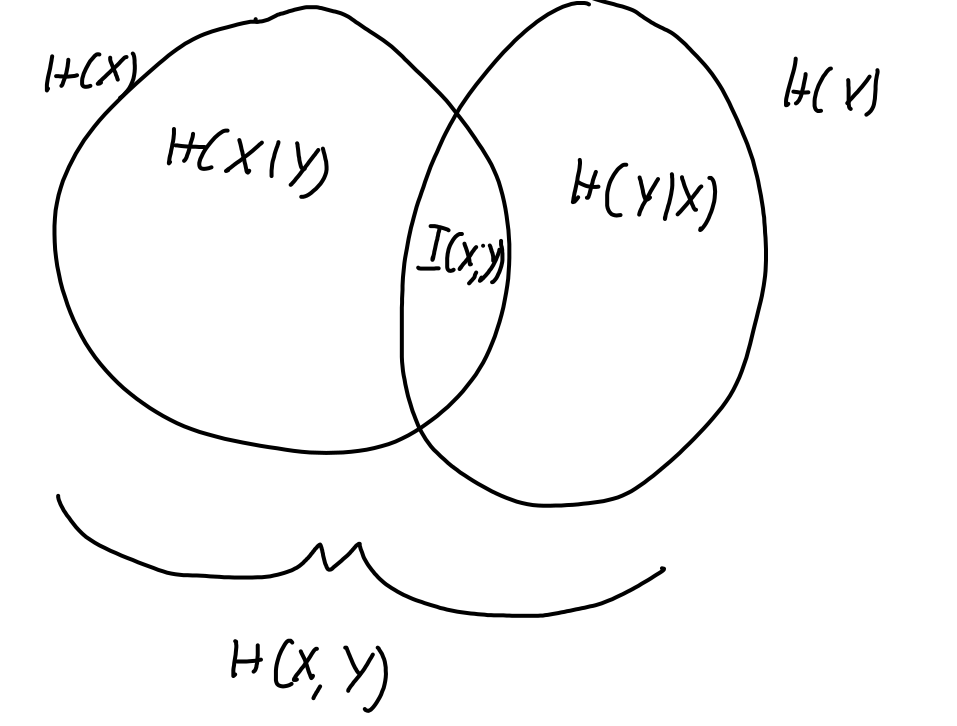
\includegraphics[scale=0.3]{venn}

  \item
    If $A$ is the event that a person lives beyond the age of 70, and $M$ is the event that you are a man, then we are interested in $p(M|A)$.

    Since old women outnumber old man by three to one, $p(M|A) = 0.25$, so the information gained by learning this event is $-\log_2 0.25 = 2$ bits.

  \item
    By Shannon's Source Coding Theorem, we know that the shortest possible code length in bits per average symbol is given by the entropy of the source:

    $\frac{1}{2} \cdot 1 + \frac{1}{4} \cdot 2 + \frac{1}{8} \cdot 3 + \frac{1}{16} \cdot 4 + \frac{1}{32} \cdot 5 + \frac{1}{32} \cdot 5 = 1.9375$ bits.

  \item
    It is more effective to improve the signal to noise ratio. When we define capacity, we use $B\log(1 + \frac{S_p}{BN_p})$, where $S_p$ and $N_p$ are signal power and noise power respectively. Increasing the bandwidth $B$ only improve the transmission capacity up to an asymptote, so we get harsh diminishing returns, whereas by improving the signal to noise ratio $\frac{S_p}{N_p}$, we can improve the capacity to any extent.

  \item
    By Nyquist's Sampling Theorem, we must sample at twice the frequency which appears in our signal, so we must sample at 2 kHz, to be able to reconstruct our signal perfectly.

    This gives us $2000 \cdot 10 = 20000$ samples.

  \item
    Not relevant.




        
\end{enumerate}
\end{document}
